% 简洁风格：浅色背景 + 细边框 + 行号 + 自动换行
\definecolor{codebg}{RGB}{248,249,250}
\definecolor{codeframe}{RGB}{220,223,228}
\definecolor{codekw}{RGB}{25,85,145}
\definecolor{codecm}{RGB}{90,125,90}
\definecolor{codestr}{RGB}{136,44,136}

\lstdefinestyle{cleancpp}{
	language=C++,
	basicstyle=\ttfamily\small,
	keywordstyle=\bfseries\color{codekw},
    commentstyle=\color{codecm},
	stringstyle=\color{codestr},
	backgroundcolor=\color{codebg},
	frame=single,
	rulecolor=\color{codeframe},
	framesep=6pt,
	numbers=left,
	numberstyle=\scriptsize\color{gray},
	numbersep=8pt,
	breaklines=true,
	breakatwhitespace=false,
	showstringspaces=false,
	keepspaces=true,
	tabsize=4,
	columns=fullflexible
}


% Start here
\chapter{Exercise 2.1}

\section{Problem}

Given the following grammar:

\begin{lstlisting}[style=cleancpp]
S -> ( L ) | a
L -> L , S | S
\end{lstlisting}

Construct a parse tree for the sentence:

\begin{lstlisting}[style=cleancpp]
(a, ((a, a), (a, a)))
\end{lstlisting}

\section{Solution}

To solve this problem, I start by analyzing the structure of the given sentence and how it can be reduced according to the grammar rules. 
After reducing the sentence step by step, we can construct the parse tree as follows:

\begin{figure}[htbp]
    \centering
    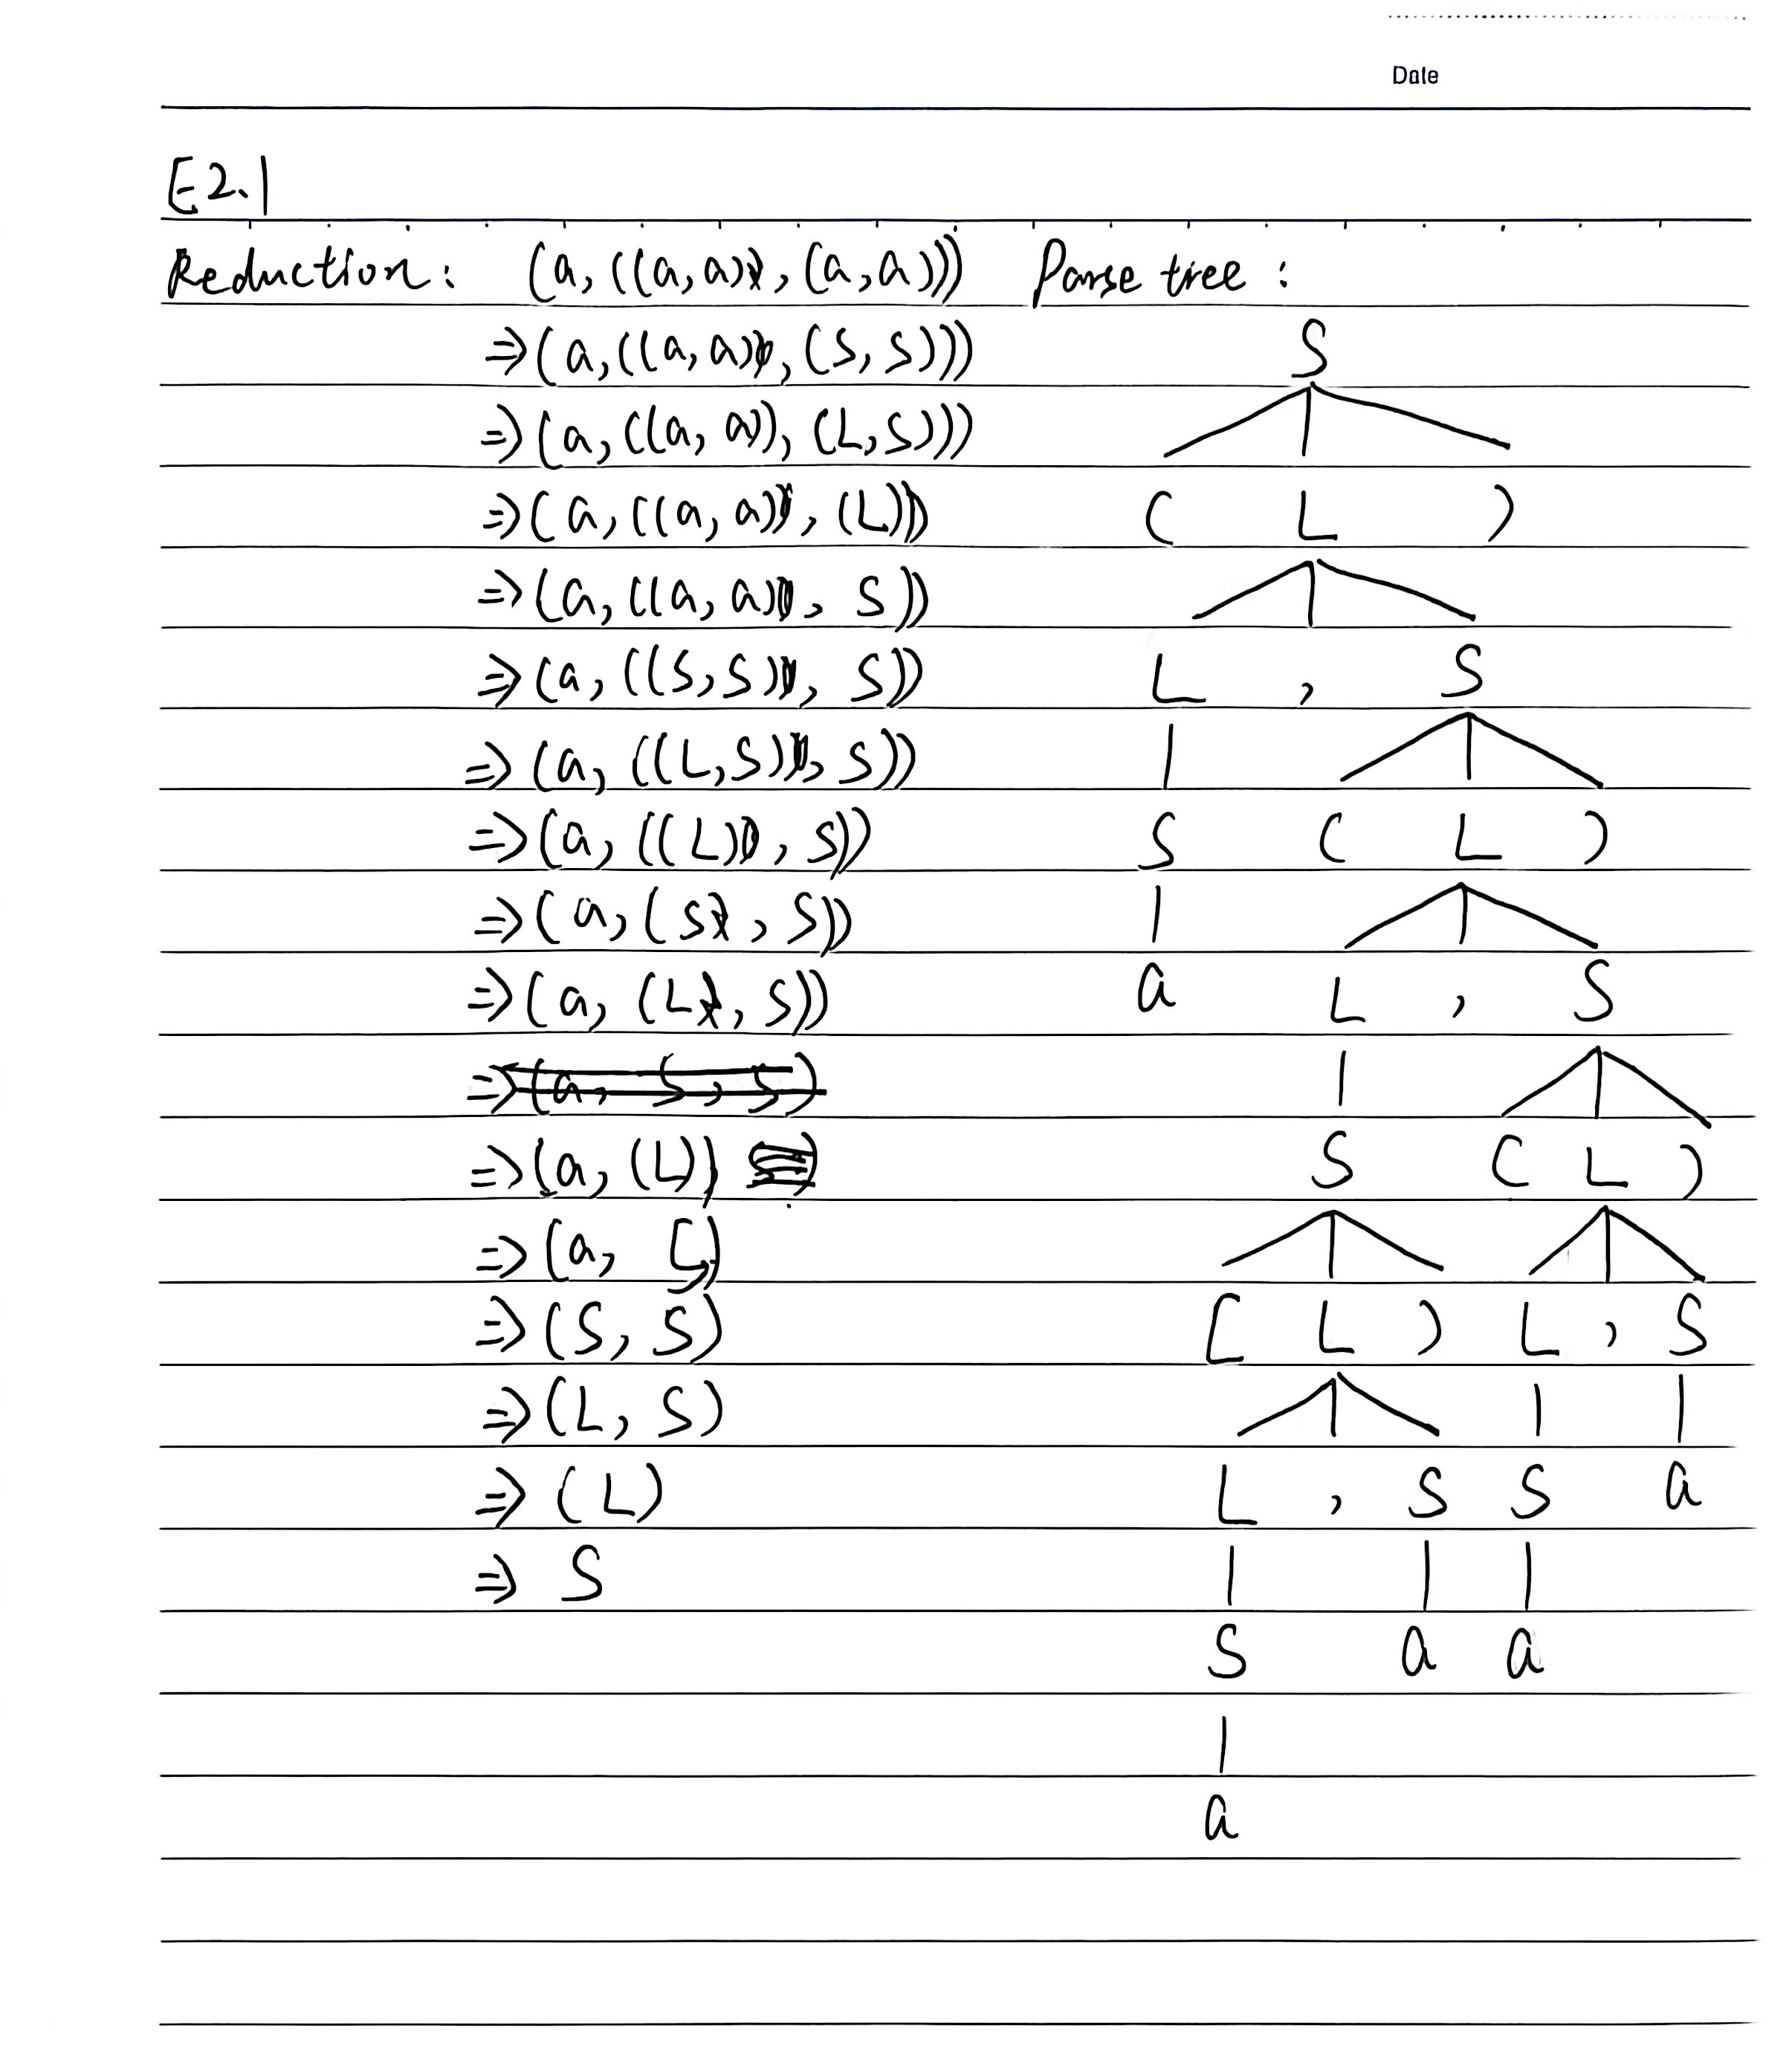
\includegraphics[width=0.6\textwidth]{image/e2_1.JPG}
\end{figure}

\chapter{Exercise 2.2}
\section{Problem}

Given the following grammar:

\begin{lstlisting}[style=cleancpp]
bexpr -> bexpr or bterm | bterm
bterm -> bterm and bfactor | bfactor
bfactor -> not bfactor | ( bexpr ) | true | false
\end{lstlisting}

Construct a parse tree for the sentence:

\begin{lstlisting}[style=cleancpp]
not (true or false)
\end{lstlisting}

\section{Solution}

\begin{figure}[htbp]
    \centering
    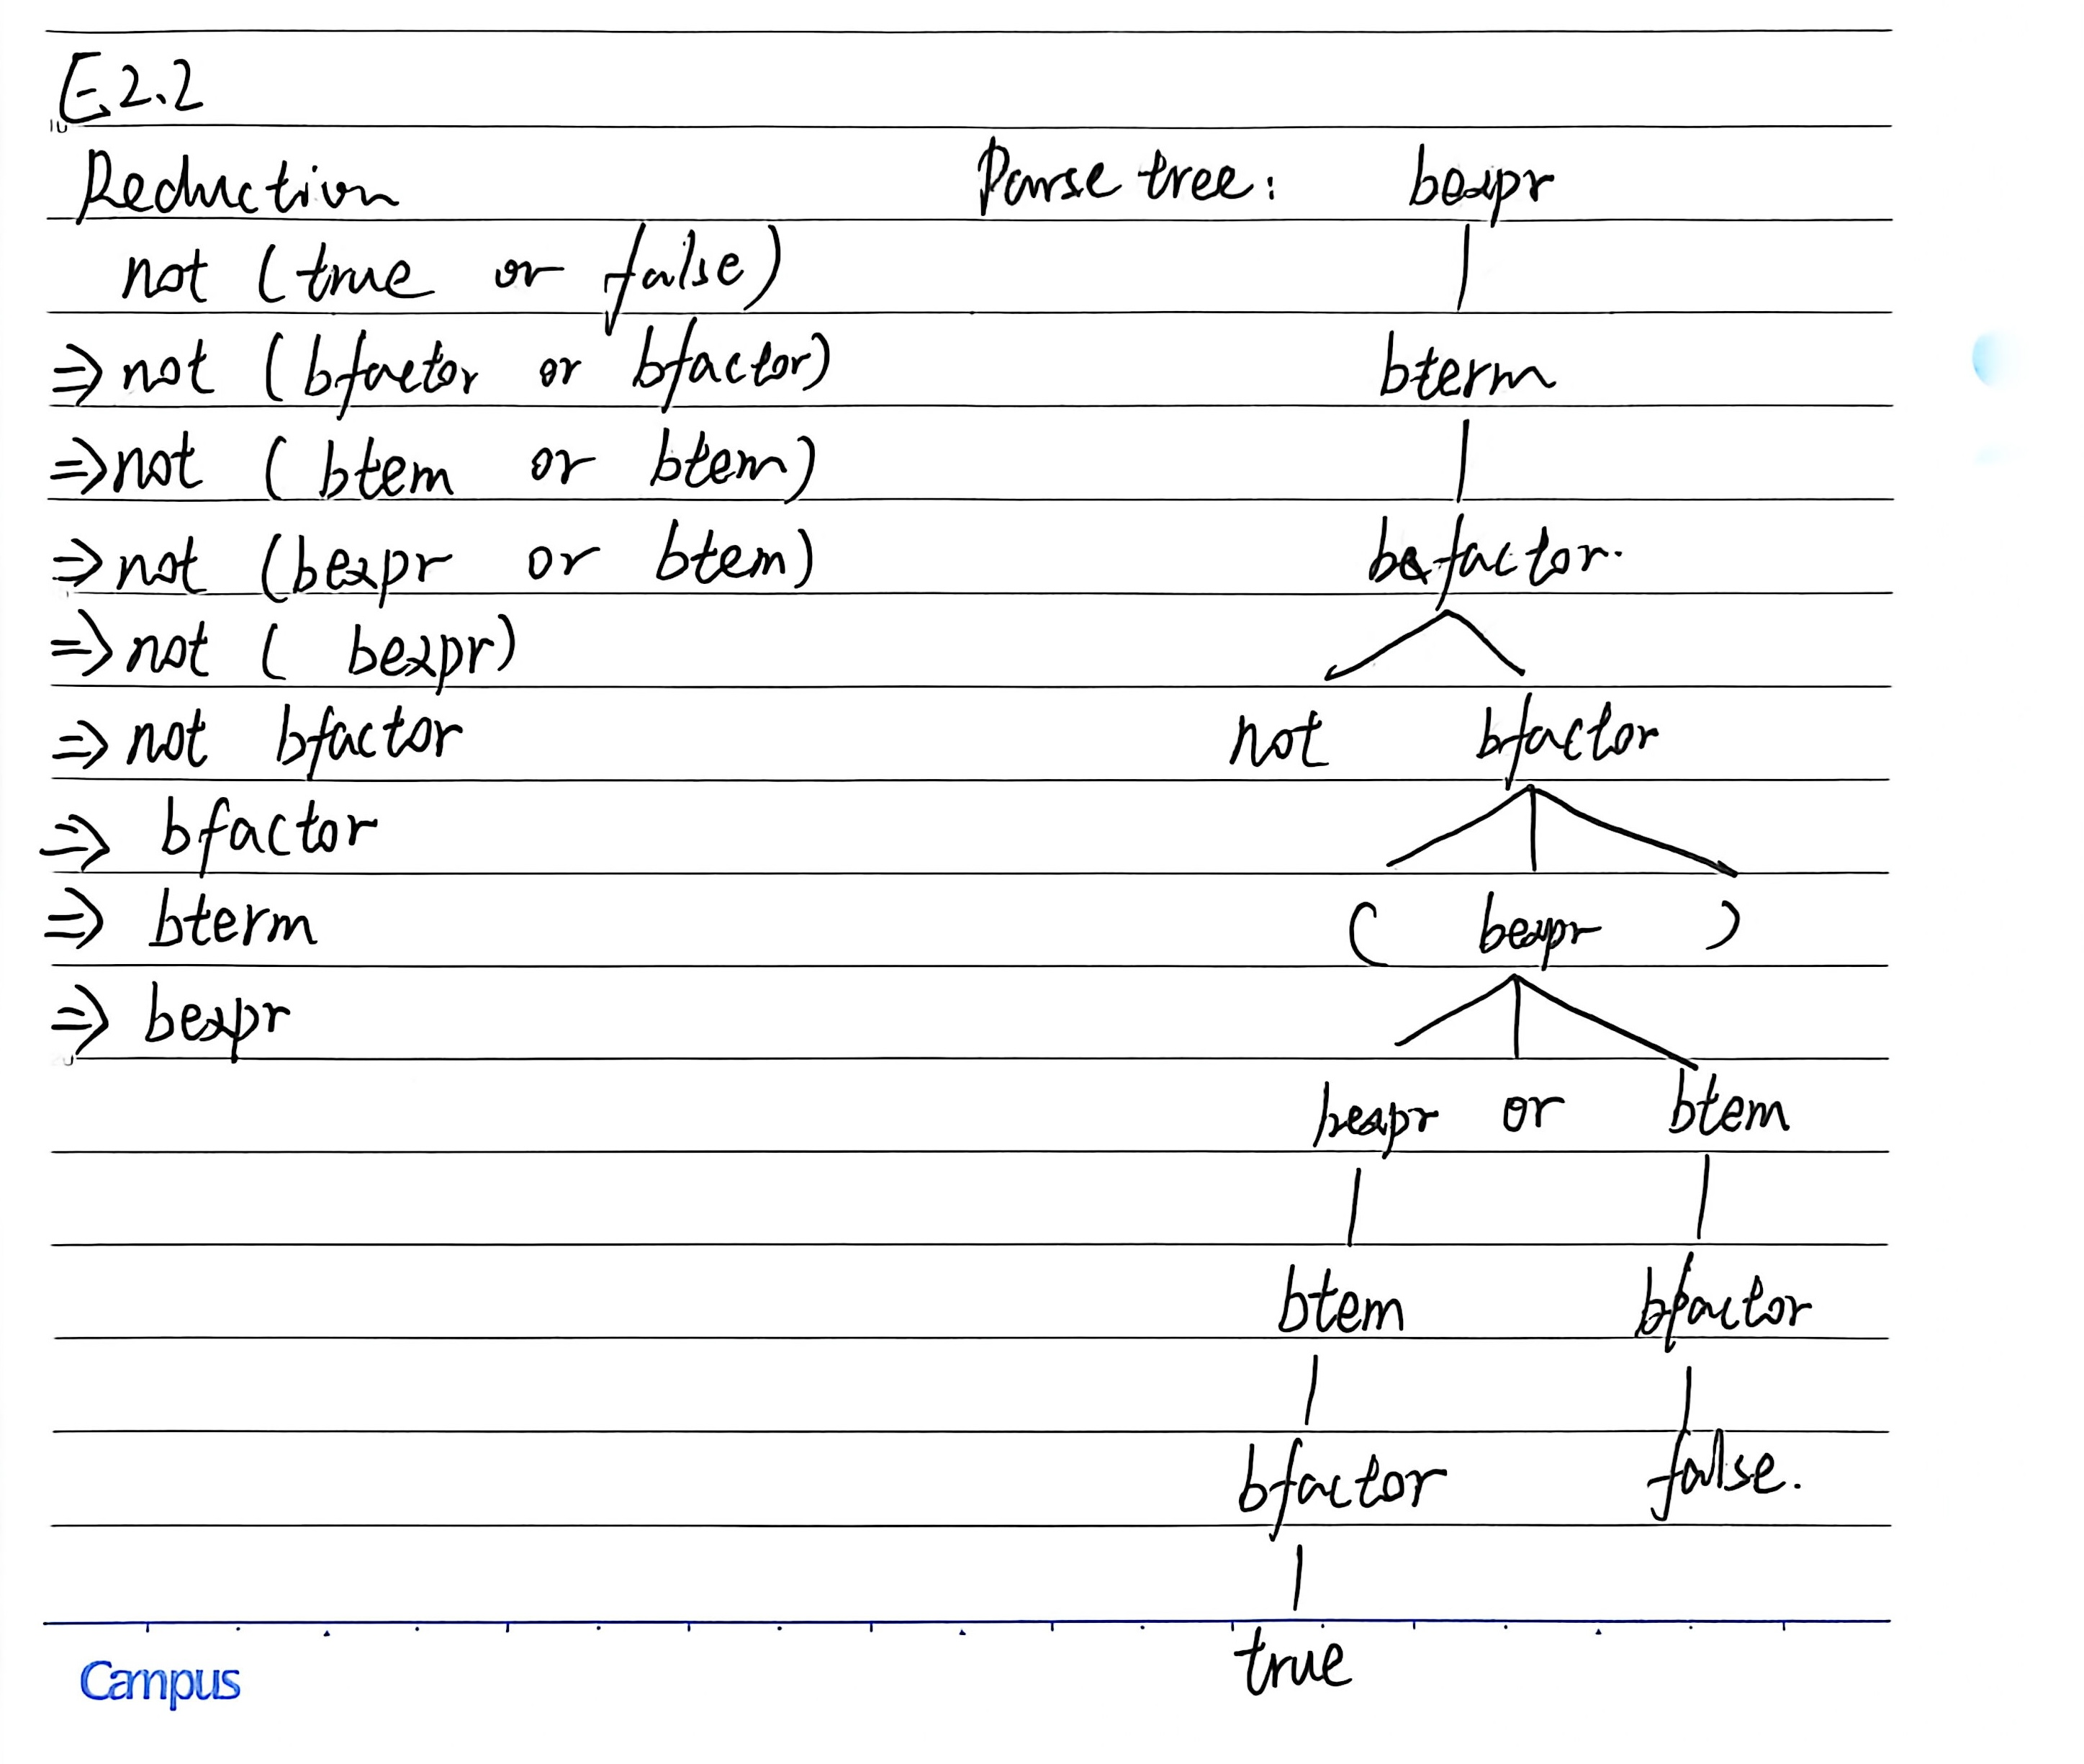
\includegraphics[width=\textwidth]{image/e2_2.JPG}
\end{figure}

\chapter{Exercise 2.3}
\section{Problem}

Is the grammar

\begin{lstlisting}[style=cleancpp]
S -> a S b S | b S a S | epsilon
\end{lstlisting}

ambiguous? Why?

\section{Solution}

Yes, the grammar is ambiguous. 
This is because there are multiple ways to derive the same string using the production rules. 

For example, there two different ways:
\begin{lstlisting}[style=cleancpp]
a b epsilon a epsilon b epsilon
a epsilon b epsilon a b epsilon
\end{lstlisting}

Both of these derivations produce the same "S".

\begin{figure}[htbp]
    \centering
    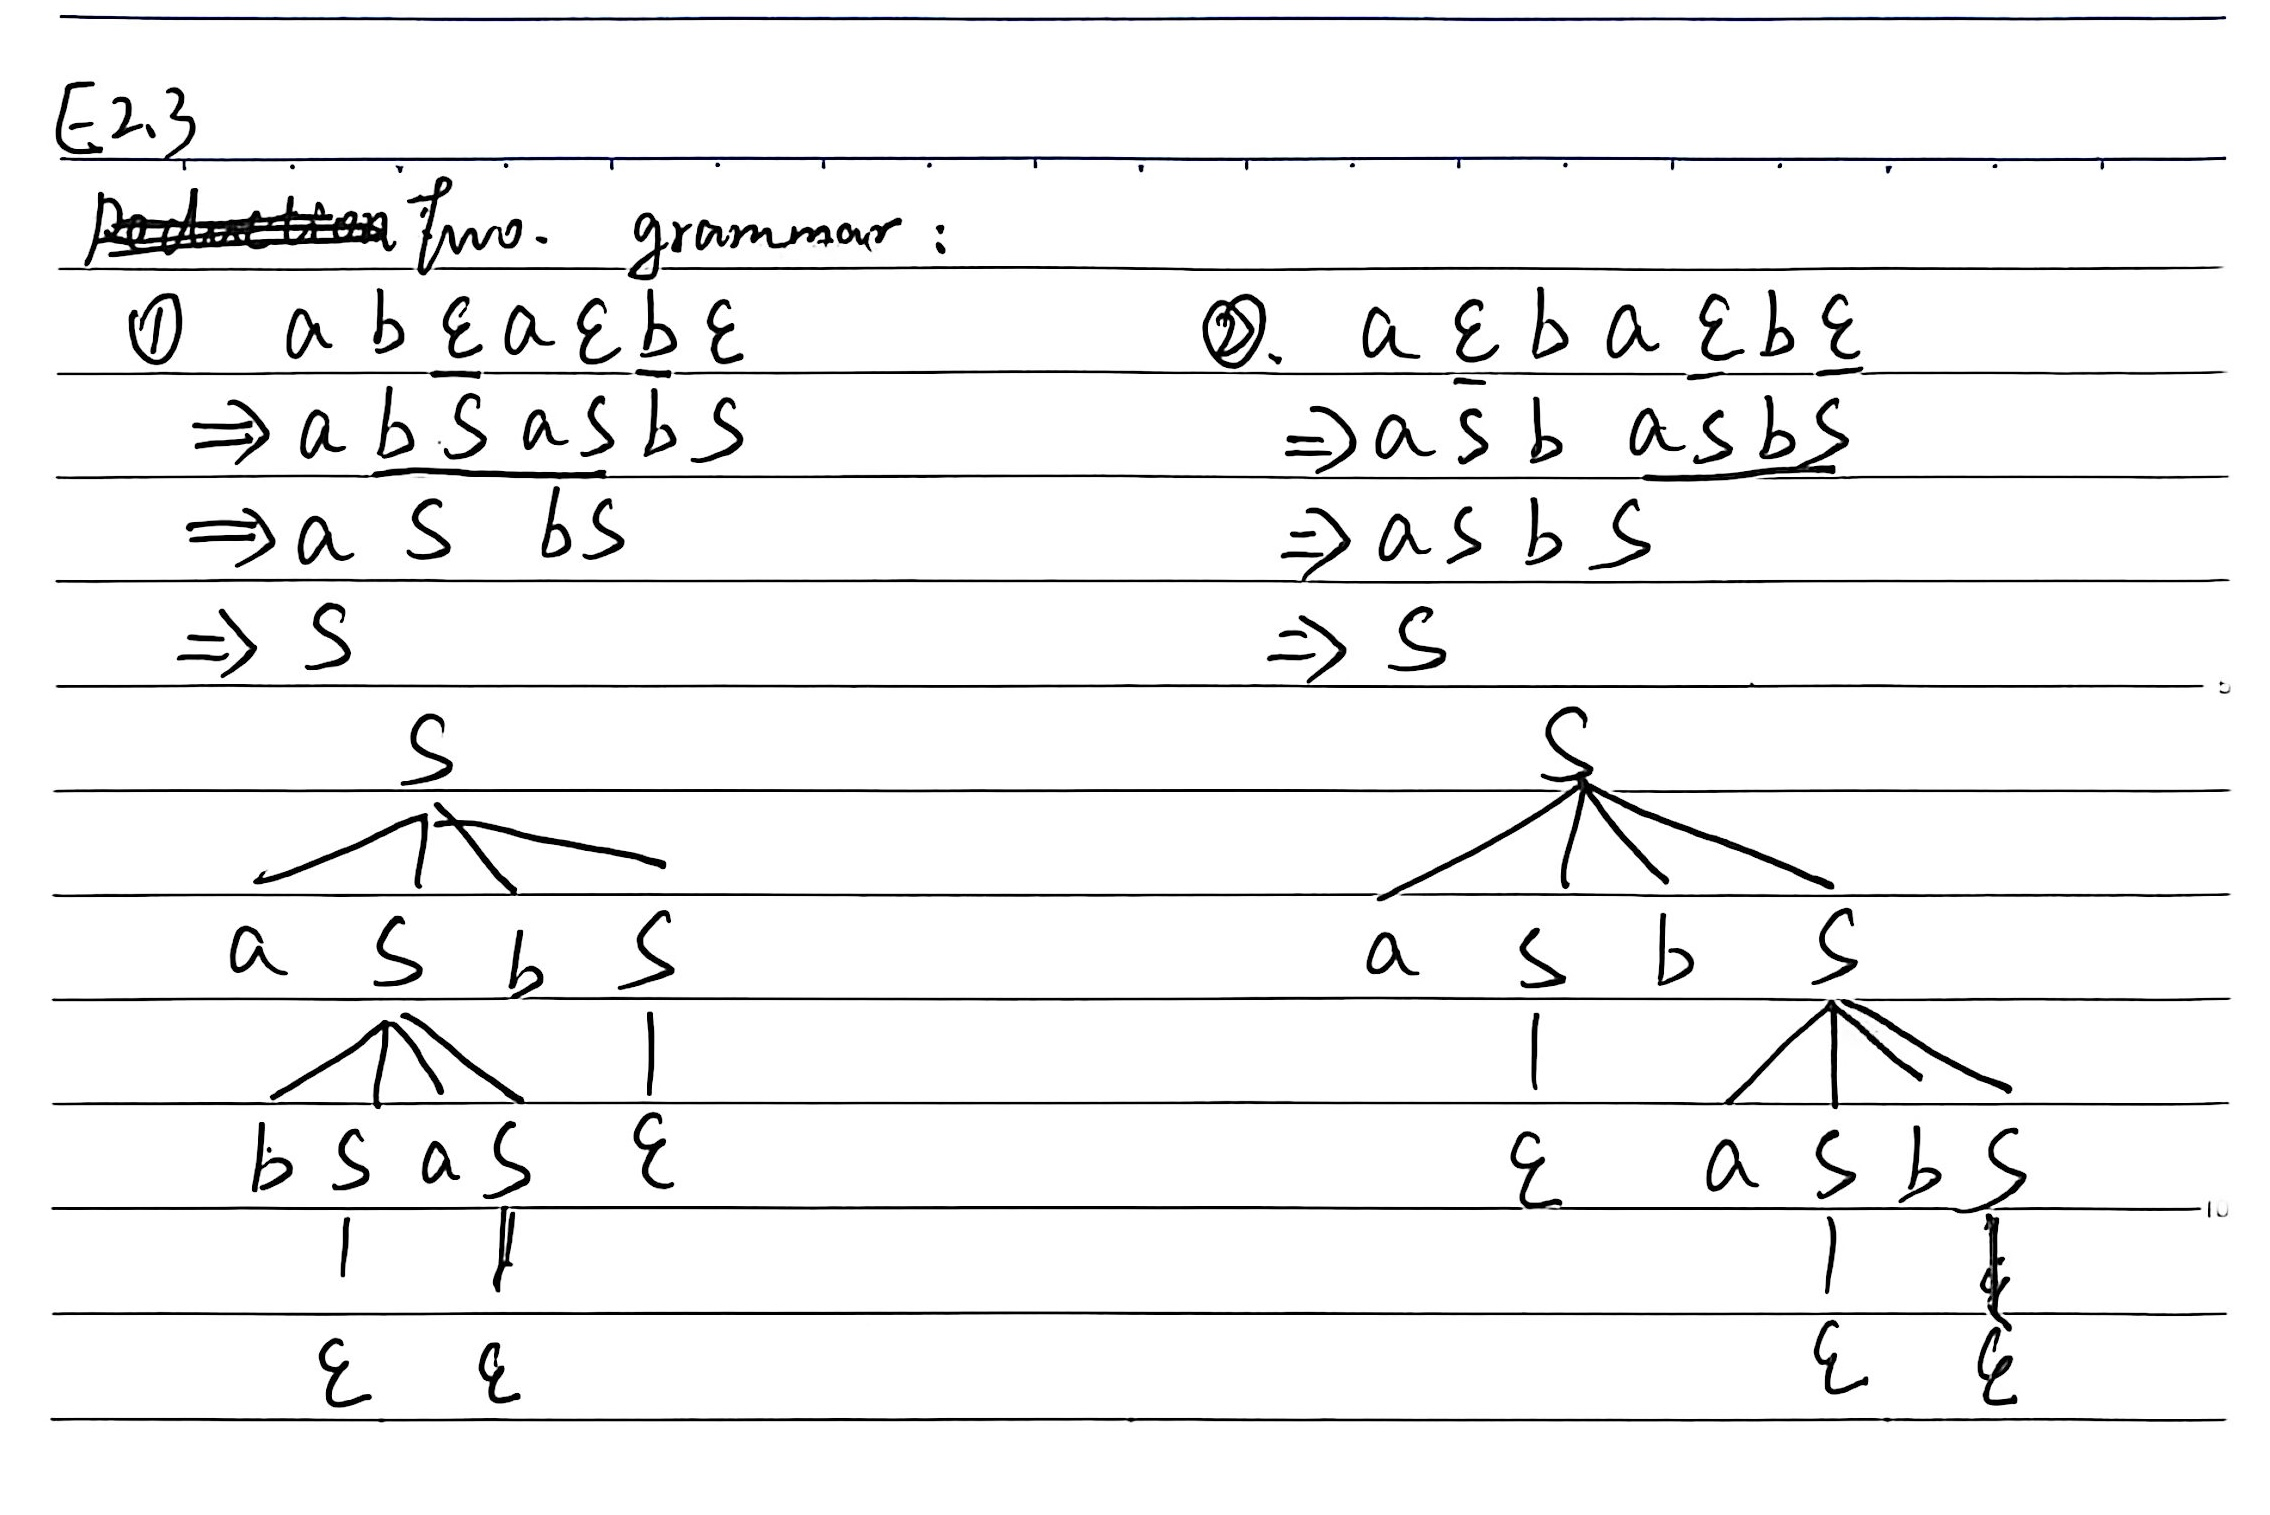
\includegraphics[width=\textwidth]{image/e2_3.JPG}
\end{figure}
